\subsection{1}
\begin{enumerate}
  \item[\text{a})]  $yu_{xx}+2u_{xy}+xu_{yy}-u_{y}=5x;$ \\
    \noindent\begin{minipage}{0.5\textwidth}
  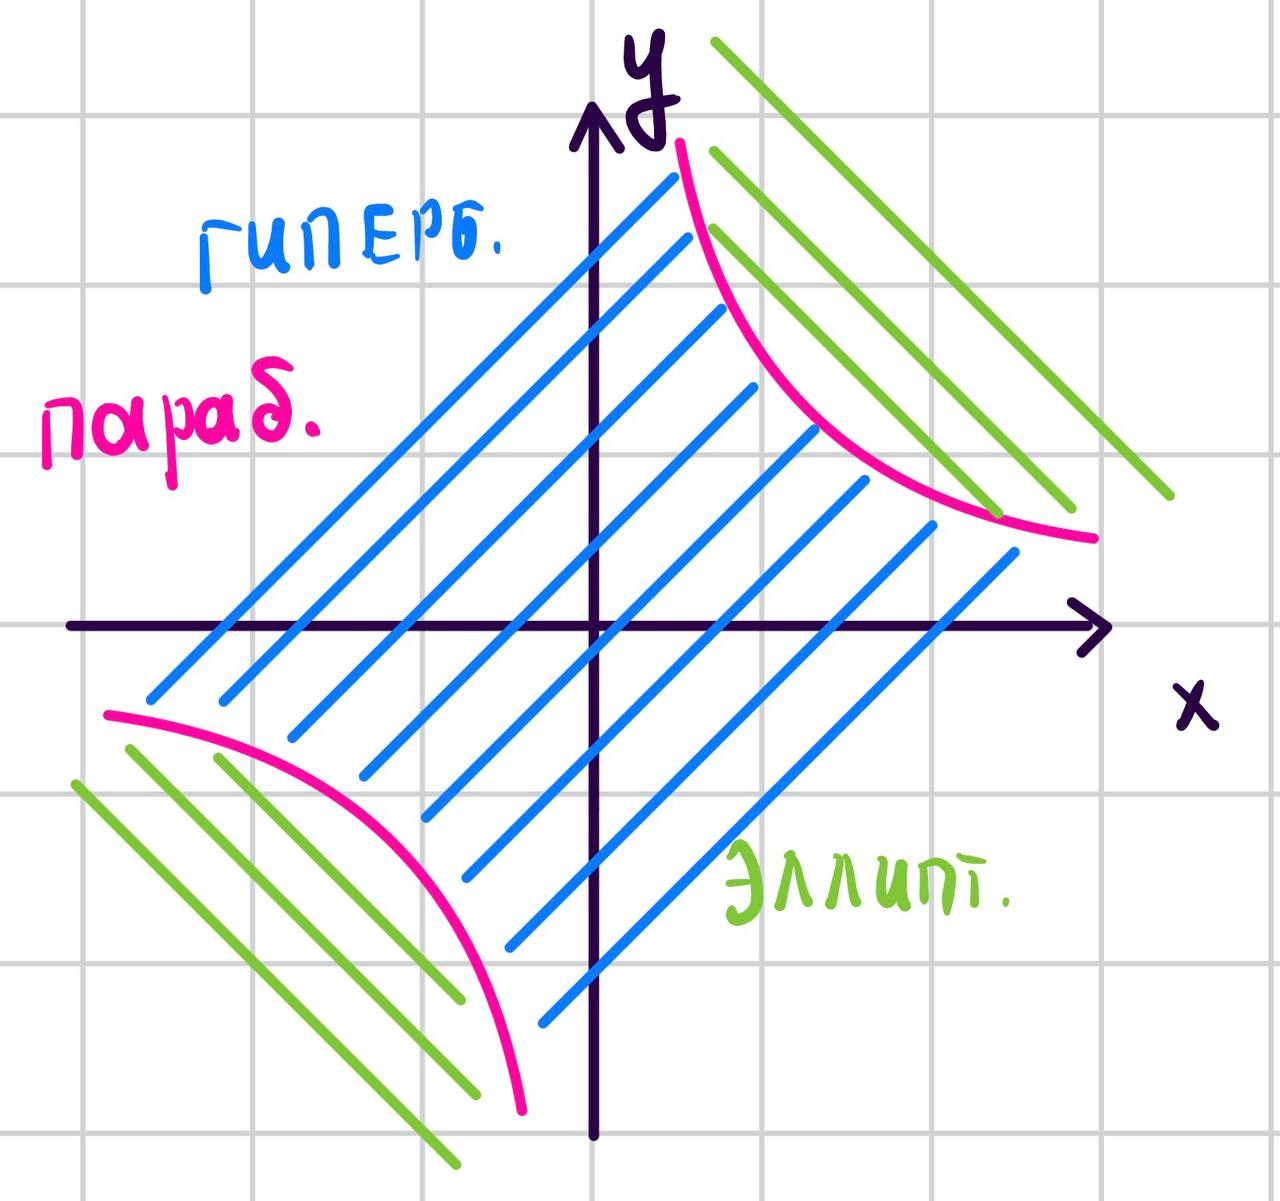
\includegraphics[width=1\linewidth]{pictures/u1.jpg} 
\end{minipage}
\hfill
\begin{minipage}{0.6\textwidth}\raggedleft
\begin{align*}
&\begin{pmatrix}
  y & 1 \\
  1 & x \\
\end{pmatrix} \\
&\Delta_{1} = y, \Delta_{2}=xy-1 \\
&\text{Эллиптический, если} \\ 
& \begin{cases}
 y > 0\\ xy-1>0 \\ 
\end{cases} \text{либо} \begin{cases}
  y < 0\\ xy-1>0
\end{cases}\\
&\text{Гиперболический, если} \\ 
& \begin{cases}
 y < 0 \\ xy-1<0 \\ 
 \end{cases} \text{ либо } \begin{cases}
  y>0 \\ xy-1<0
\end{cases}\\
&\text{Параболлический, если} \\
&xy-1=0 \\ 
\end{align*}
\end{minipage}
\newpage
\item[\text{б})] $(x^{2}+y^{2}-1)u_{xx}+xyu_{yy}-u_{x} = 0.$ \\
  \begin{minipage}{0.3\textwidth}
  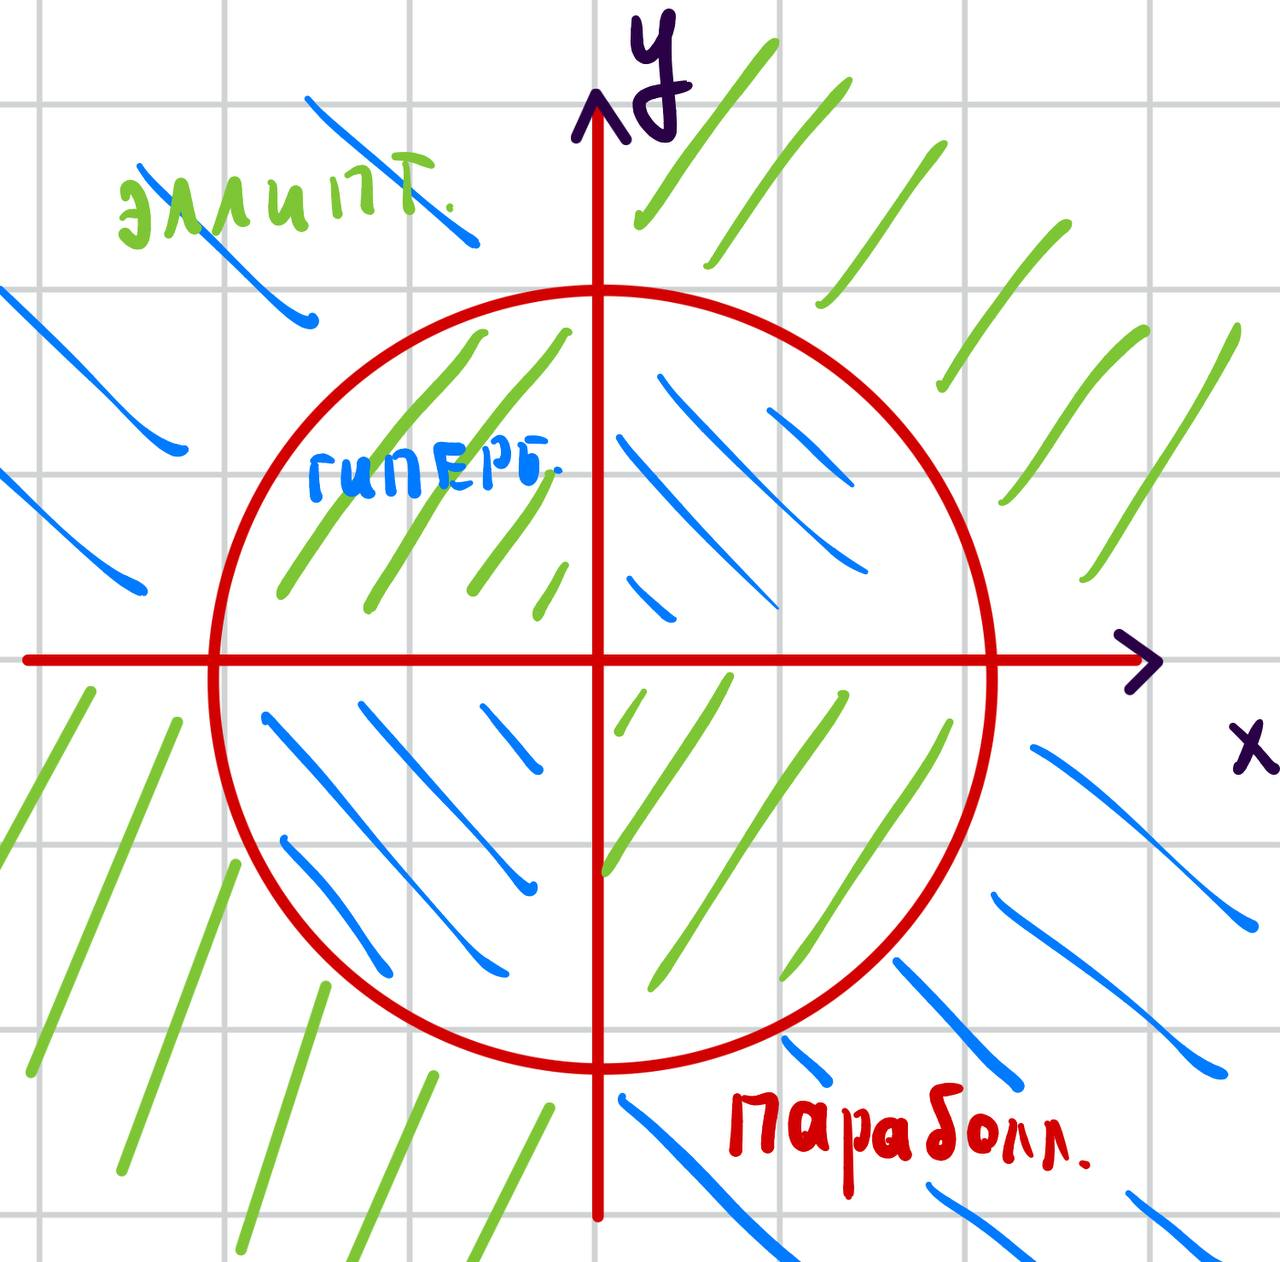
\includegraphics[width=1.3\linewidth]{pictures/u2.jpg} 
  \end{minipage}
  \begin{minipage}{0.6\textwidth}\raggedleft
\begin{align*}
&\begin{pmatrix}
x^{2}+y^{2}-1 & 0 \\
0 & xy \\
\end{pmatrix} \\
&\text{Эллиптический, если} \\ 
&xy(x^{2}+y^{2}-1) > 0\\
&\text{Гиперболический, если} \\ 
&xy(x^{2}+y^{2}-1) < 0\\
&\text{Параболлический, если} \\ 
&xy(x^{2}+y^{2}-1) = 0\\
\end{align*}
  \end{minipage}
\end{enumerate}
\subsection{2} 
$u_{xx}+2\alpha u_{xz}+u_{yy}+4\beta u_{yz}+4u_{zz}=0.$ \\
  \begin{minipage}{0.3\textwidth}
  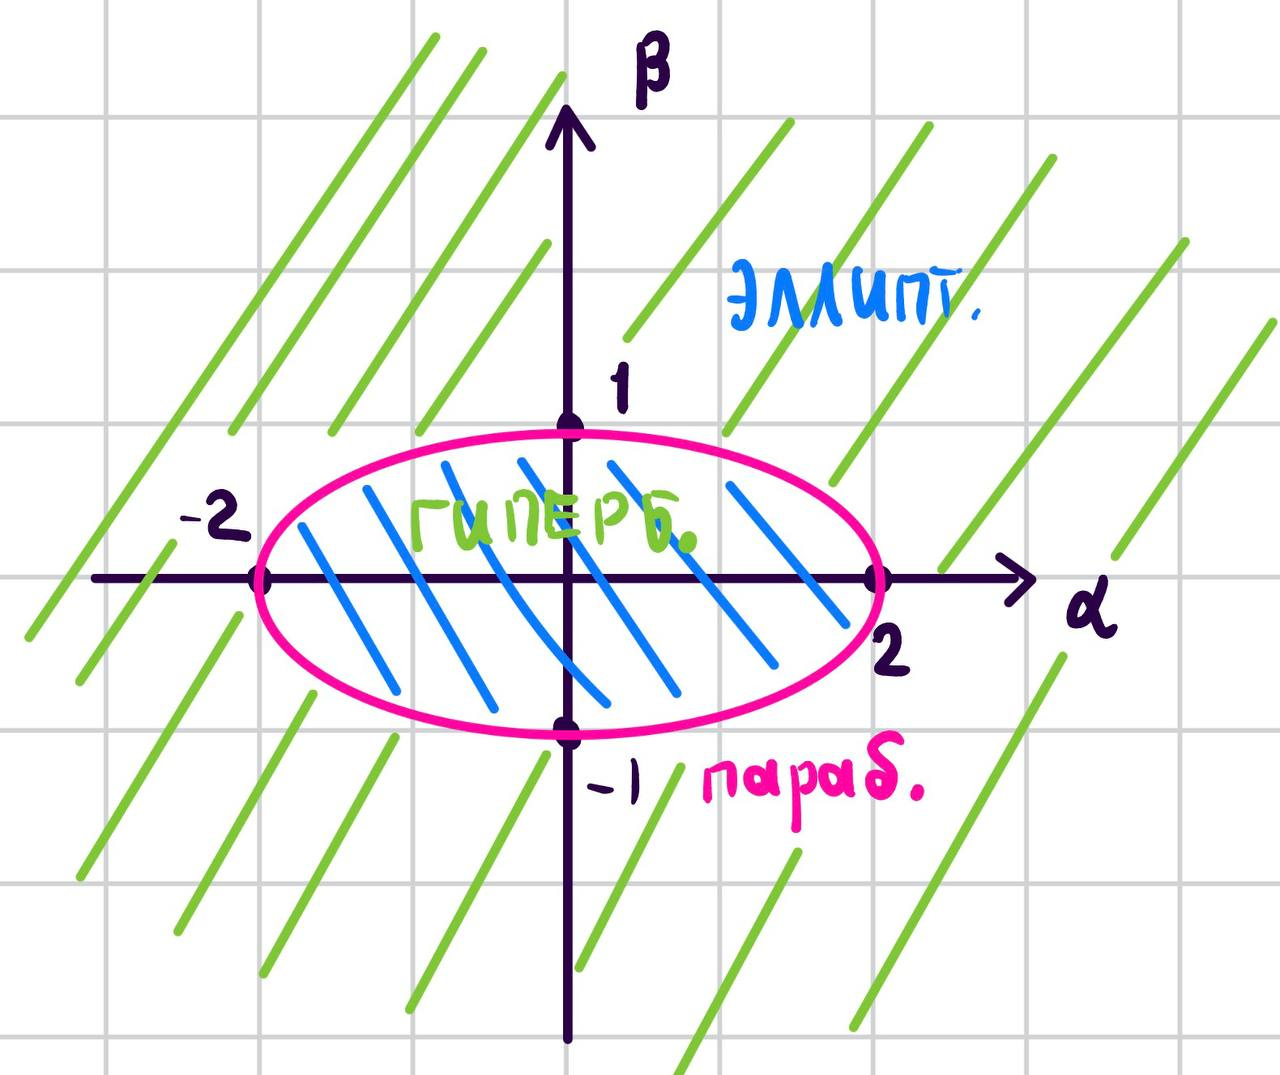
\includegraphics[width=1.4\linewidth]{pictures/u3.jpg} 
  \end{minipage}
  \begin{minipage}{0.6\textwidth}\raggedleft
\begin{align*}
&\begin{pmatrix}
  1 & 0&\alpha \\
  0&1&2\beta \\ 
  \alpha&2\beta&4 \\
\end{pmatrix} \\
&\Delta_{3}=4-4\beta^{2}-\alpha^{2}\\
&\text{Эллиптический, если} \\ 
&4-4\beta^{2}-\alpha^{2}>0\\
&\text{Гиперболический, если} \\ 
&4-4\beta^{2}-\alpha^{2}<0\\
&\text{Параболлический, если} \\ 
&4-4\beta^{2}-\alpha^{2}=0\\
\end{align*}
  \end{minipage}
\subsection{2.1(2)}
$4u_{xx}-4u_{xy}-2u_{yz}+u_{y}+u_{z}=0$
\begin{align*}
&  \left(4 \frac{\partial^{2}}{\partial x^{2}}-4 \frac{\partial^{2}}{\partial x\partial y}-2
  \frac{\partial^{2}}{\partial y\partial z} \right)u+u_{y}+u_{z}=0 \\
 & \left( \left(\underbrace{2\frac{\partial}{\partial x}
    -\frac{\partial}{\partial y}}_{ \frac{\partial}{\partial\xi}}\right)^{2}-\left( 
    \underbrace{\frac{\partial}{\partial y}
 +\frac{\partial}{\partial z}}_{ \frac{\partial}{\partial \mu}}\right)^{2}+\left( \underbrace{
\frac{\partial}{\partial z}}_{ \frac{\partial}{\partial \nu}}\right)^{2}\right)u
  +u_{y}+u_{z}=0\\
 & u_{\xi\xi}-u_{\mu \mu}+u_{\nu \nu}+u_{\mu}=0 \quad \text{гиперболический} \\
 & u = u(x(\xi,\mu\nu),y(\xi,\mu,\nu),z(\xi,\mu,\nu)) \\
 & \frac{\partial u}{\partial \xi} = \frac{\partial u}{\partial x}\underbrace{\frac{\partial x}{\partial \xi}}_{2}+
 \frac{\partial u}{\partial y}\underbrace{\frac{\partial y}{\partial \xi}}_{-1}+
 \frac{\partial u}{\partial z}\underbrace{\frac{\partial z}{\partial \xi}}_{0} \\
 & \frac{\partial u}{\partial \mu} = \frac{\partial u}{\partial x}\underbrace{\frac{\partial x}{\partial \mu}}_{0}+
 \frac{\partial u}{\partial y}\underbrace{\frac{\partial y}{\partial \mu}}_{1}+
 \frac{\partial u}{\partial z}\underbrace{\frac{\partial z}{\partial \mu}}_{1} \\
 & \frac{\partial u}{\partial \nu} = \frac{\partial u}{\partial x}\underbrace{\frac{\partial x}{\partial \nu}}_{0}+
 \frac{\partial u}{\partial y}\underbrace{\frac{\partial y}{\partial \nu}}_{0}+
 \frac{\partial u}{\partial z}\underbrace{\frac{\partial z}{\partial \nu}}_{1} \\
 & \text{Замена} \\
 & \begin{cases}
   x = 2\xi \\ y =-\xi + \mu \\ z = \mu + \nu \\ 
  \end{cases} \\
\end{align*}

